
% !TEX encoding = latin1
% !TEX TS-program = pdflatex
% !TEX root = ../handout_qft.tex
% !TEX spellcheck = it-IT

%*******************************************************
% Chapter 1
%*******************************************************

\myChapter{Schwinger's own way to teach quantum mechanics}
%\myChapter{Schwinger's approach to quantum mechanics}
\label{chp:fundamentals} 

%\minitoc\mtcskip

\begin{refsection}
\begin{quoting}
   \openquote 
   I presume that all of you have already been exposed to some undergraduate
   course in Quantum Mechanics, one that leans heavily on de Broglie waves and
   the Schroedinger equation. I have never thought that this simple wave
   approach was acceptable as a general basis for the whole subject, and I
   intend to move immediately to replace it in your mind by a foundation that
   \emph{is} perfectly general.~\closequote
   \begin{flushright}
       J. Schwinger,
       \emph{Quantum Mechanics. Symbolism of Atomic Measurements}
       \textcite{Schwinger:2001}.
    \end{flushright}
\end{quoting}

\section{Introduction}

\lettrine{I}{n} 
comparisong to other areas of physics, quantum mechanics presents unique challenges.
On one hand, quantum theory stands as a great reminder of how intuition can be misleading and untrustworthy.
 In particular, the intuitions developed from classical physics prove insufficient in offering the guidance necessary to grasp the intricacies of the quantum world.
  On the other hand, the mathematical machinery required to adeguately formulate quantum mechanics carries a substantial initial complexity, and it can contribute to obfuscate some of the physical implications, or at least it represents a technical distraction from the main area of focus. 

  One might wonder: is this level of mathematical sophistication required from the start?
  As it will become clearer soon, the inherent properties of quantum systems --- 
  such as Heisenberg's uncertanty principle, probabilistic outcome of 
 quantum measurements, entanglement, and superposition of quantum
  states --- demand alternative mathematical abstractions capable of accommodating 
such properties.  The traditional mathematical tooling empowered by classical physics 
  proven inadeguate to 
capture such phenomena, naturally driving the search for alternative formalisms.

  Remarkably enough, quantum mechanics not only triggered a shift in perspective about our understanding of physics, but also forced to revisit the \emph{mathematical infrastructure} needed to organise, support, and encode properties and behaviours of quantum systems.


For example, as it will be discussed in depth, incompatibility between physical measurable quantities like position and
momentum, which is at the root of uncetainty principle, can be described in
terms of \emph{non-commutative} objects, leading to adopt some sort of non-commuting mathematical entity like 
operators instead of real numbers to describe position and momentum.
Similarly, 
  the canonical commutation relations impose further
constrains: as they can't be realised in finite-dimensional linear spaces,
  they force to work with infinite-dimensional spaces. 

Is it possible to circumvent the use of Hilbert space?
As we proceed towards the final chapters,
  alternative formulations will be provided, notably
  the path integral approach to quantum mechanics due to Richard Feynman. This approach has pros and cons, it's somehow better suited to be generalised to quantum field theory, and offers physical insights, but it still requires a degree of mathematical sophistication. We will also see how the language of category theory can remove some of the noise of the Hilbert space formulation and really allow to reveal some of the underlying core concepts (at the price of more advanced mathematical sophistication). 

  In \cref{chap:rules}, the mathematical principles of non-relativistic quantum mechanics are presented systematically using the language of Hilbert spaces. These postulates, crystallized during the 1920s and 1930s, emerged after few decades of intense and captivating endeavors by the pioneering minds of quantum mechanics. This period witnessed substantial advancements in theory and experimentation, intertwined with missteps, erroneous attempts, and an array of intellectual pursuits. Although contemporary students might readily adopt these postulates as a foundation to develop the theory, the historical context often obscures the original motivations behind this formulation.

  In this chapter, a complementary path to introduce quantum mechanics is discussed.
This inspiring approach, due to Schwinger and presented in \textcite{Schwinger:2001}, 
supplements  the content in \cref{chap:rules} by providing physical intuitition, insights, and motivation behind those postulates.

% Navigando a vista in un mare allora sconosciuto, inciampando negli
% imprevisti, 
% un percorso di intuizioni poi dimostratesi erronee, tentativi andati a vuoto
% vicoli ciechi, intuizioni che hanno spronato direzioni importanti per poi non
% trovare posto nella costruzione definitiva. 
% Questo lavoro e' confluito e si riassume nei postulati della meccanica
% quantistica.
% La loro validita' si poggia in ultima analisi sull'accordo con i fatti  sperimentali ovviamente, come per ogni
% branca della fisica. La loro forma e' quella a cui sono approdotati coloro
% che 
% Tuttavia, l'elevato livello di astrazione che li caratterizza, puo' 



\begin{figure}
   \centering
   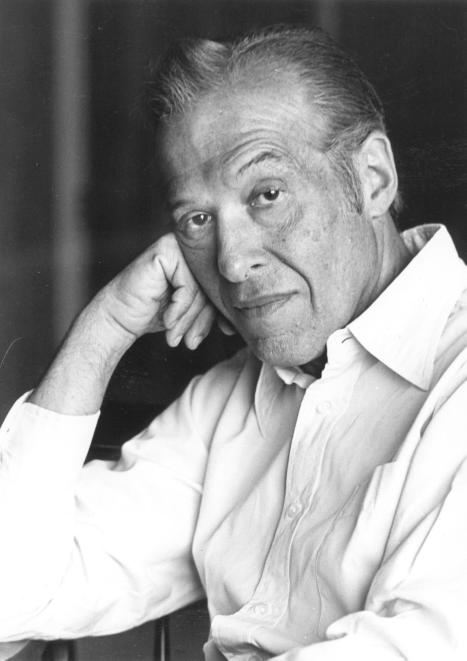
\includegraphics[scale=.35]{./Images/schwinger}
   \caption{Julian Seymour Schwinger (February 12, 1918 -- July 16, 1994) }
\end{figure}

\printbibliography[heading=subbibliography]
\end{refsection}
